\documentclass[12pt,letterpaper]{article}
\usepackage{geometry}
\usepackage{graphicx}

\geometry{
top=0.0in,
bottom=1in,
left=1in,
right=1in
}

\title{\textbf{Problem Set Six}}
\author{Devin Williams}
\date{\today}

\begin{document}

\maketitle

\begin{itemize}
    \item Data cleaning steps:
        \begin{itemize}
            \item[$\diamond$] Step One: Remove unneeded columns
                \begin{itemize}
                     \item[$\diamond$] This data set came with multiple unneeded columns for analysis. Including the rank, fee in pounds, and reference list columns. These were removed using the select function in R. 
                \end{itemize}
                \item[$\diamond$] Step Two: Change column names
                \begin{itemize}
                     \item[$\diamond$] Multiple other columns did not have a descriptive title. These include the "Fee in Euros" column as well as the "New" and "Old" club columns having their names changed from "fee..million", "to", and "from". This was done using the mutate function. 
                \end{itemize}
             \item[$\diamond$] Step Three: Convert column type
                \begin{itemize}
                     \item[$\diamond$] The newly changed "Fee in Euros" was not considered a numeric variable, causing some issues with ggplot2. The column was changed and the euro symbol was removed. 
                \end{itemize}
             \item[$\diamond$] Step Four: Create "League Type" column
                \begin{itemize}
                     \item[$\diamond$] A new column was added to use for a later plot. "League type" was created by creating a vector that mapped the teams in the data set to their leagues. This was then added to the new column. 
                \end{itemize}
             \item[$\diamond$] Step Five: One last variable
                \begin{itemize}
                     \item[$\diamond$] Finally, the "max fee" variable was created to be used in another plot. This allowed the maximum fee to be shown on the graph in plot 2. 
                \end{itemize}
         \end{itemize}
\end{itemize}

\newpage %Added before each visualization to allow for everything about each graph to appear on one page together
\vspace*{2cm}
\begin{itemize}
    \item First visualization:
        \begin{figure}[h!]  
            \centering
            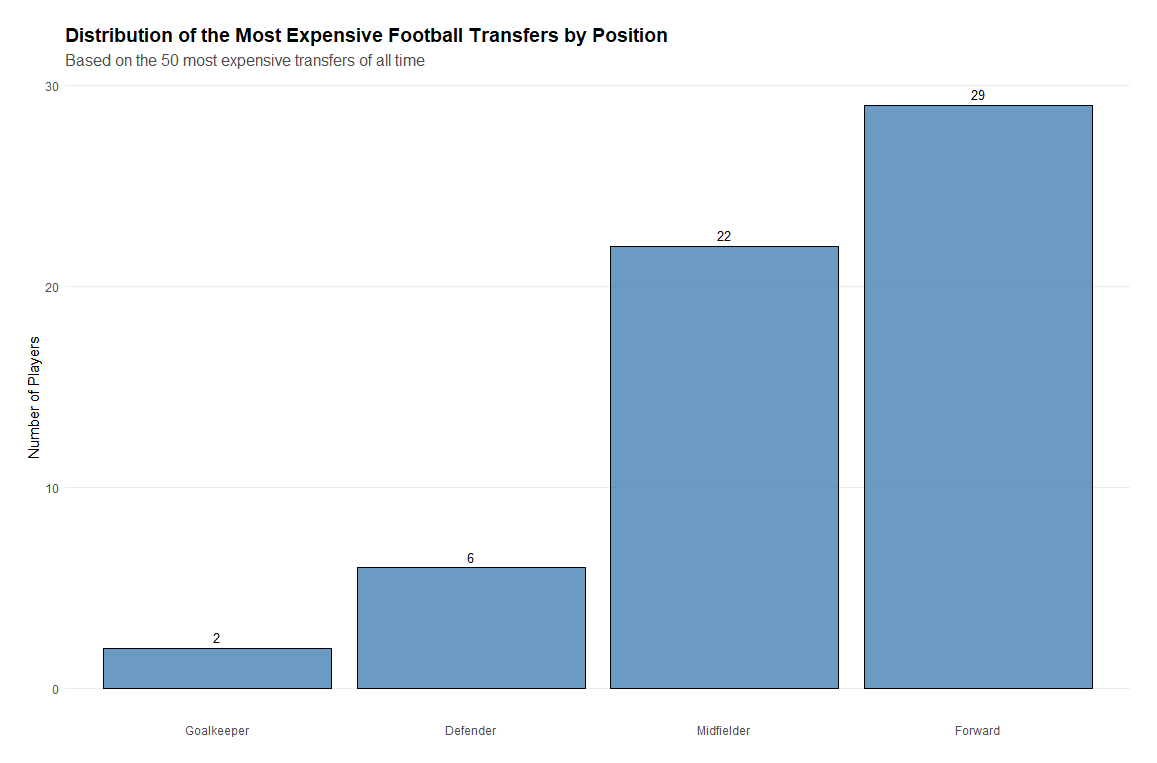
\includegraphics[width=1\textwidth]{PS6a_Williams.png}
        \end{figure}
            \begin{itemize}
            \item[$\diamond$] This image communicated how many of the top 50 most expensive transfers play each position. This is helpful to understand what world football teams spend money on, and how the trend continues to favor more attacking players. 
             \end{itemize}
\end{itemize}
\newpage
\vspace*{2cm}
\begin{itemize}
    \item Second visualization:
        \begin{figure}[h!]  
            \centering
            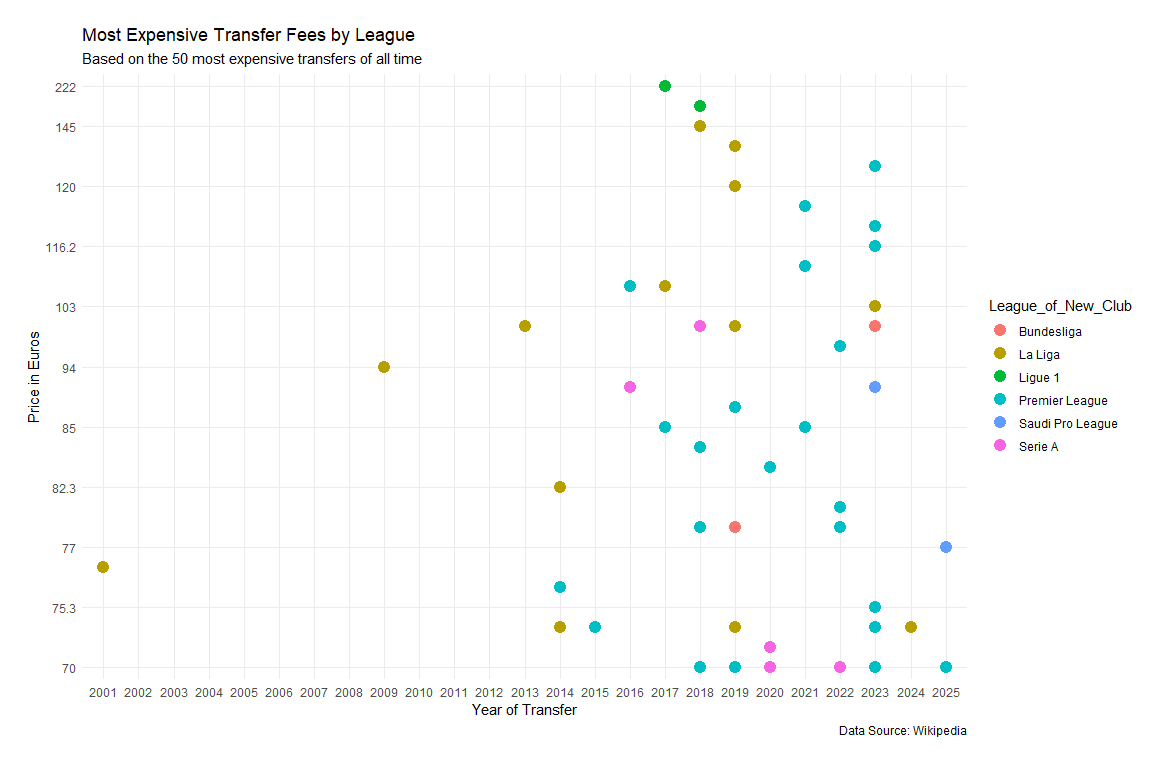
\includegraphics[width=1\textwidth]{PS6b_Williams.png}
        \end{figure}
            \begin{itemize}
            \item[$\diamond$] This image both demonstrates the continued high spending of world football, as well as getting a look at how the premier league has come to dominate financially. This looks to communicated the most expensive transfer fees by year, while also looking at which leagues made these signings. 
             \end{itemize}
\end{itemize}
\newpage
\vspace*{2cm}
\begin{itemize}
    \item Third visualization:
        \begin{figure}[h!]  
            \centering
            \includegraphics[width=1\textwidth]{PS6C_Williams.png}
        \end{figure}
            \begin{itemize}
            \item[$\diamond$] This graph takes a closer look at the top three top years for transfers. This again shows the trend towards more spending, while showing which years had the most top 50 transfers of all time. 
             \end{itemize}
\end{itemize}

\end{document}
